\documentclass[tikz]{standalone}
\usepackage{pgfplots}
\pgfplotsset{compat=1.18}
\begin{document}
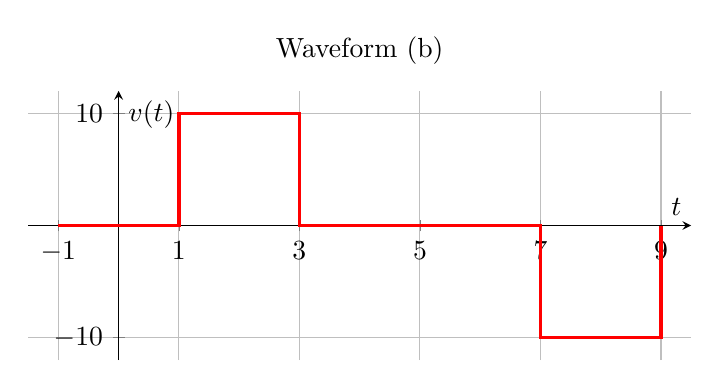
\begin{tikzpicture}
\begin{axis}[
    axis lines = middle,
    xlabel = {$t$},
    ylabel = {$v(t)$},
    xmin = -1.5, xmax = 9.5,
    ymin = -12, ymax = 12,
    xtick = {-1, 0, 1, 3, 5, 7, 9},
    ytick = {-10, 0, 10},
    grid = both,
    width=10cm, height=5cm,
    title = {Waveform (b)}
]
\addplot[red, very thick, no marks] coordinates {
    (-1, 0) (1, 0)
    (1, 10) (3, 10)
    (3, 0) (7, 0)
    (7, -10) (9, -10)
    (9, 0) % End of period T=8 starting from t=1
};
\end{axis}
\end{tikzpicture}
\end{document}
